
\item The figure shows a system consisting of (i) a ring of outer radius \(3R\) rolling clockwise without slipping on a horizontal surface with angular speed \(\omega\) and (ii) an inner disc of radius \(2R\) rotating anti-clockwise with angular speed \(\omega/2\). The ring and disc are separated by frictionless ball bearings. The system is in the \(x-z\) plane. The point \(P\) on the inner disc is at a distance \(R\) from the origin, where \(OP\) makes an angle of \(30^\circ\) with the horizontal. Then with respect to the horizontal surface,
    \begin{center}
        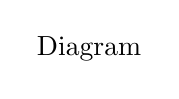
\begin{tikzpicture}
            \node at (0, 0) {Diagram};
        \end{tikzpicture}
    \end{center}
    \begin{tasks}(1)
        \task the point \(O\) has a linear velocity \(3R\omega \mathbf{i}\).
        \task the point \(P\) has a linear velocity \(\frac{11}{4} R\omega \mathbf{i} + \frac{\sqrt{3}}{4} R\omega \mathbf{k}\).
        \task the point \(P\) has a linear velocity \(\frac{13}{4} R\omega \mathbf{i} - \frac{\sqrt{3}}{4} R\omega \mathbf{k}\).
        \task the point \(P\) has a linear velocity \(\left(3 - \frac{\sqrt{3}}{4}\right) R\omega \mathbf{i} + \frac{1}{4} R\omega \mathbf{k}\).
    \end{tasks}
